\documentclass[11pt,leqno]{article}
\headheight=13.6pt

% packages
\usepackage[alphabetic]{amsrefs}
\usepackage{physics}
% margin spacing
\usepackage[top=1in, bottom=1in, left=0.5in, right=0.5in]{geometry}
\usepackage{hanging}
\usepackage{amsfonts, amsmath, amssymb, amsthm}
\usepackage{systeme}
\usepackage[none]{hyphenat}
\usepackage{fancyhdr}
\usepackage{graphicx}
\graphicspath{{./images/}}
\usepackage{float}
\usepackage{siunitx}
\usepackage{esint}
\usepackage{color}
\usepackage{enumitem}
\usepackage{mathrsfs}
\usepackage{hyperref}
\usepackage[noabbrev, capitalise]{cleveref}
\crefformat{equation}{equation~#2#1#3}
\crefformat{lemma}{\textrm{Lemma}~#2#1#3}
\usepackage{hanging}

% theorems
\theoremstyle{plain}
\newtheorem{lem}{Lemma}
\newtheorem{lemma}[lem]{Lemma}
\newtheorem{thm}[lem]{Theorem}
\newtheorem{theorem}[lem]{Theorem}
\newtheorem{prop}[lem]{Proposition}
\newtheorem{proposition}[lem]{Proposition}
\newtheorem{cor}[lem]{Corollary}
\newtheorem{corollary}[lem]{Corollary}
\newtheorem{conj}[lem]{Conjecture}
\newtheorem{fact}[lem]{Fact}
\newtheorem{form}[lem]{Formula}

\theoremstyle{definition}
\newtheorem{defn}[lem]{Definition}
\newtheorem{definition/}[lem]{Definition}
\newenvironment{definition}
  {\renewcommand{\qedsymbol}{\textdagger}%
   \pushQED{\qed}\begin{definition/}}
  {\popQED\end{definition/}}
\newtheorem{example}[lem]{Example}
\newtheorem{remark}[lem]{Remark}
\newtheorem{exercise}[lem]{Exercise}
\newtheorem{notation}[lem]{Notation}

\numberwithin{equation}{section}
\numberwithin{lem}{section}

% header/footer formatting
\pagestyle{fancy}
\fancyhead{}
\fancyfoot{}
\fancyhead[L]{M 382D}
\fancyhead[C]{HW6}
\fancyhead[R]{Sai Sivakumar}
\fancyfoot[R]{\thepage}
\renewcommand{\headrulewidth}{1pt}

% paragraph indentation/spacing
\setlength{\parindent}{0cm}
\setlength{\parskip}{10pt}
\renewcommand{\baselinestretch}{1.25}

% extra commands defined here
\newcommand{\br}[1]{\left(#1\right)}
\newcommand{\sbr}[1]{\left[#1\right]}
\newcommand{\cbr}[1]{\left\{#1\right\}}
\newcommand{\eq}[1]{\overset{(#1)}{=}}

% bracket notation for inner product
\usepackage{mathtools}

\DeclarePairedDelimiterX{\abr}[1]{\langle}{\rangle}{#1}

\DeclareMathOperator{\Span}{span}
\DeclareMathOperator{\im}{im}
\newcommand{\res}[1]{\operatorname*{res}_{#1}}
\DeclareMathOperator{\id}{id}
\DeclareMathOperator{\Hom}{Hom}
\DeclareMathOperator{\Adj}{Adj}
\DeclareMathOperator{\Ad}{Ad}
\DeclareMathOperator{\End}{End}
\DeclareMathOperator{\codim}{codim}
\DeclareMathOperator{\Int}{int}
\newcommand{\GL}{\mathrm{GL}}
\newcommand{\Mat}{\mathrm{M}}
\newcommand{\Sp}{\mathrm{Sp}}
\newcommand{\AS}{\mathrm{AntiSym}}

% set page count index to begin from 1
\setcounter{page}{1}

\begin{document}
I worked on this problem set with Sudharshan KV.
\begin{enumerate}
    \item Let $Y = \mathbb R^2$, $X = \mathbb H^2$ (the closed upper half plane in $\mathbb R^2$), and $Z$ the graph of $H(x)(\pi-x)\exp(-1/x^2)$ where $H$ is the Heaviside step function (i.e. characteristic function of $\cbr{x\geq 0}$), pictured below.
    \begin{center}
        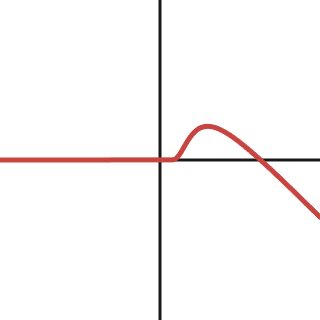
\includegraphics[width=10em]{Z.png}
    \end{center}
    The inclusion of $X$ in $Y$ is transverse to $Z$, but the inclusion of the horizontal axis is not transverse to $Z$, in particular on the non-positive real axis. The preimage of $X\cap Z$ along the inclusion of $X$ in $Y$ is the set $\cbr{(x,0)\mid x\leq 0}\cup \cbr{(\pi,0)}$, which cannot be a manifold since it is the disjoint union of a point and an open interval.
    \item We showed in class that the self intersection number mod $2$ of $Z_1$ with itself is $1$. We show that the intersection number of $Z_2$ with itself is zero by perturbing $Z_2$ slightly: 
    
    Consider the $1$-parameter family $Z_t$ in $\mathbb {RP}^2 = \cbr{[x:y:z]}$ cut out by the homogeneous polynomial $(t-1/2)yz + 2(1-t)xz = y^2$, which agrees with $Z_2$ for $t = 1/2$. But for $t>1/2$, the two points of $Z_t\cap Z_2$ are $[0:0:1]$ and $[1:2:4]$, and choose $t$ so that $Z_t$ is transverse to $Z_2$ (we should be able to do this by genericity of transversality). Therefore intersection number of $Z_2$ with itself mod $2$ is zero. Since $Z_1,Z_2$ have different self intersection numbers mod $2$, they could not be homotopic since the intersection number is homotopy invariant.
    \item \begin{enumerate}
        \item For any $y\in Y$, let $c_y\colon X \to Y$ be the constant map taking $X$ to the point $y$. Let $f$ be homotopic to the map $c_p$ for some $p\in Y$. The map $c_p$ is homotopic to a constant map $c_q$ where $q$ is not contained in $Z$: Since $Z$ has dimension strictly less than that of $Y$, in a suitable chart $(U,\phi)$ around $p$ we may choose a point $\phi(p) + \varepsilon v$ for suitably small $\varepsilon> 0$, where $v$ belongs to the orthogonal complement of the subspace of $\mathbb R^d$ that $\phi(U\cap Z)$ belongs to (we may choose $(U,\phi)$ so that $\phi(U)$ lies in a proper subspace of $\mathbb R^{\dim Y}$). Let $q = \phi^{-1}(\phi(p) + \varepsilon v)$. Postcomposing the straight-line homotopy from the constant map to $\phi(p)$ to the constant map to $\phi(p) + \varepsilon v$ with $\phi^{-1}$ produces a homotopy from $c_p$ to $c_q$. Since homotopy is an equivalence relation, $f$ is homotopic to $c_q$. Since $q$ is not contained in $Z$, $c_q$ is transverse to $Z$. Thus $I_2(f,Z) = I_2(c_q,Z) = 0\pmod 2$.
        \item Let $X$ be a compact boundaryless manifold of positive dimension and let the identity map on $X$ be homotopic to $c_p$ for some $p\in X$. Since tangent spaces of zero-dimensional manifolds are the zero vector space, $\id_X$ is transverse to $p$ so that $I_2(\id_X,\cbr{p}) = 0 \pmod{2}$ by part (a). But the preimage of $\cbr{p}$ under the identity map is $p$, so $I_2(\id_X,\cbr{p}) = 1 \pmod{2}$. Therefore $X$ could not have positive dimension as assumed, so $X$ is a discrete set of points. For $X$ to be contractible we must have that $X$ is a single point.
    \end{enumerate}
    \item \begin{enumerate}
        \item For $n = 0$ the question does not make sense and for $n = 1$ the only submanifolds of $S^1$ with positive dimension are $1$-dimensional, so assume $n\geq 2$. Two compact submanifolds $X,Z$ of $S^n$ of complimentary positive dimension cannot cover $S^n$: Both $X$ and $Z$ have to have dimension strictly less than $n$, so in particular $X$ is not equal to $S^n$. Let $p\in S^n\setminus X$ and consider the chart $(U = S^n\setminus \cbr{p},\phi)$ given by stereographic projection. Then $U$ is homeomorphic to $\mathbb R^n$ with $\phi(X)$ a compact subset of $\mathbb R^n$; that is, a closed and bounded subset of $\mathbb R^n$. If $p$ is not in $Z$, there is nothing to show. But by Sard's theorem, the image of $Z\setminus \cbr{p}$ is measure zero in $\mathbb R^n$, so there must exist points away from $X$ and $Z$ in $S^n$. Choose $q\in S^n\setminus (X\cup Z)$ and consider stereographic projection away from $q$. We may homotope the images of $X$ and $Z$ under this projection so that they are disjoint; by pulling the homotopy back along the projection, it follows that $X$ and $Z$ are homotopic to non-intersecting compact subsets of $S^n$, so $I_2(X,Z) = 0\pmod 2$.
        \item Let $M$ and $N$ both have positive dimension and identify $M$ and $N$ as submanifolds of $M\times N$ via the inclusions $i_{n_0}\colon M \to M\times N$ sending $m$ to $(m,n_0)$ and $j_{m_0}$ defined similarly for $N$. The intersection of $M$ and $N$ in $M\times N$ is $1\pmod 2$, and the intersection number is invariant under diffeomorphism, so $S^n$ could not be diffeomorphic to any such $M\times N$. If now one of $M$ or $N$ has dimension zero, then $S^n$ cannot be diffeomorphic to $M\times N$ if the dimension zero manifold has more than one point, since $S^n$ is connected. Thus $S^n$ may only be diffeomorphic to $M\times N$ if one of them is a point (and so the other has to be diffeomorphic to $S^n$).
        \item Consider the embeddings of $\mathbb {RP}^1$ and $\mathbb {RP}^{n-1}$ in $\mathbb {RP}^n$ given by $[x_0:x_1]\mapsto [x_0:\cdots:x_1]$ and $[x_0:x_{n-1}]\mapsto [x_0:\cdots:x_{n-1}:0]$, respectively. Then the only point of intersection is the point $[1:0:\cdots:0]$. At this point in the chart $U_0$, the image of the differentials of the embeddings above are the orthogonal complements of each other in $\mathbb R^n$; they are $\cbr{(x_1,\cdots,x_{n-1},0)}$ and $\cbr{(0,\cdots,0,x_n)}$ and hence sum to $\mathbb R^n$. Therefore these compact submanifolds of $\mathbb {RP}^n$ are transverse to each other with intersection number $1\pmod 2$. This again implies that $S^n$ could not be diffeomorphic to $\mathbb {RP}^2$.
    \end{enumerate}
    \item Let $f_t\colon \mathbb {RP}^2\to \mathbb {RP}^2$ be given by $f_t([x:y:z]) = [2tx:2(1-t)y:z]$. Observe that for $t = 1/2$, $f$ is the identity map, and viewing $t$ as a parameter from $[1/2,3/4]$, for example, can be used to define a homotopy of the identity. Therefore the graphs of $f_t$ for $t$ in this interval are homotopic. The graph of $f_{3/4}$ denoted $\Gamma(f_{3/4})$ is transverse to graph $\Delta$ of the identity: The point of intersection of $\Delta$ and $\Gamma(f_{3/4})$ is $p = ([0:0:1],[0:0:1])$. In the chart $U_2\times U_2$, the tangent spaces at $p$ in coordinates are the span of the columns of $\bigg(\!\begin{smallmatrix}
        1 & 0 \\ 0 & 1 \\ 1 & 0 \\ 0 & 1
    \end{smallmatrix}\!\bigg)$ (for $\Delta$) and $\bigg(\!\begin{smallmatrix}
        1 & 0 \\ 0 & 1 \\ 3/2 & 0 \\ 0 & 1/2
    \end{smallmatrix}\!\bigg)$, which together sum to $\mathbb R^4$. Hence the intersection number mod $2$ of $\Delta$ with itself is the intersection number mod $2$ of $\Delta$ with $\Gamma(f_{3/4})$, which is $1\pmod 2$.
    \item Let $f_0$ and $f_1$ be bordant in $Y$ via $F\colon W\to Y$. Perturb $F$ so that it is transverse to $Z$ while also preserving the transversality of $f_0,f_1$ with $Z$. Then by the generalized preimage theorem, $F^{-1}(Z)$ is a (compact) submanifold of $W$ of dimension $1$ with boundary given by $F^{-1}(Z)\cap (X_0\sqcup X_1) = (F^{-1}(Z)\cap X_0)\sqcup (F^{-1}(Z)\cap X_1) = f_0^{-1}(Z)\sqcup f_1^{-1}(Z)$. Since $X_0,X_1$ are compact, $f_0^{-1}(Z)$ and $f_1^{-1}(Z)$ are finite. The number of points in $f_0^{-1}(Z)$ differ from $f_1^{-1}(Z)$ by a multiple of two (e.g. if $F^{-1}(Z)$ has a part that leaves $X_0$ and returns to $X_0$ instead of going to $X_1$) since $F^{-1}(Z)$ is compact. Hence $I_2(f_0,Z) = I_2(f_1,Z)$.
    
    Consider $X\sqcup X$ and the smooth map $c_y\sqcup f: X\sqcup X\to Y$, where $c_y$ is the constant map to some $y\in Y$. This map may be extended to a smooth map $F\colon W\sqcup W\to Y$ where $F$ on the first $W$ is the constant map $c_y$ and is the extension of $f$ to $W$ provided by assumption. Therefore $c_y$ is bordant to $f$ in $Y$. Assume $\dim X$ is positive. For any submanifold $Z$ of complimentary dimension to $X$ in $Y$, choose $y$ away from $Z$ ($Z$ has strictly smaller dimension than $Y$) so that $c_y$ is transverse to $Z$, and without loss of generality, assume (by perturbing) that $f$ is transverse to $Z$. Therefore by the first part we have $0 \pmod 2 = I_2(c_y, Z) = I_2(f,Z)$.

    If $\dim X$ is zero, then the number of points in $X$ is even since it is the boundary of a compact $1$-dimensional manifold. In this case $c_y$ is automatically transverse to $Z$, and we repeat the above argument. Since the number of points in $X$ is even, $0 \pmod 2 = I_2(c_y, Z) = I_2(f,Z)$. 
    \item \begin{enumerate}
        \item Let $Y = \mathbb R^2$, let $Z = \cbr{(x,0)\mid \abs{x} < 1}$ and let $X = S^1$ centered at $(1,0)$ be given by $\{(x,y)\mid (x-1)^2+y^2=1\}$. Presently $X$ is transverse to $Z$ and intersects once, but homotoping $X$ away by changing its center yields zero intersections.
        \item Interchange $X$ with $Z$ in (a), and homotope the interval away from the circle to lose the single intersection via homotopy.
        \item The example in (a) with $W$ the closed disk centered at $(1,0)$ works since the inclusion of the circle into $Y$ extends to the inclusion of the disk into $Y$.
        \item If $X$ is not compact, then $W$ could not be compact since $X$ is closed in $W$. If $X$ is the horizontal axis in $\mathbb R^2$, then choosing $W$ to be the closed upper half plane $\mathbb H^2$ and by including $X$ into $\mathbb R^2$, $I_2(X,X)$ is not well defined (not homotopy invariant).
        \item Let $Y = S^1\times \mathbb R$, $X = S^1\times \cbr{0}$, $Z = \cbr{p}\times\mathbb R$ for any fixed $p\in S^1$. Then $X$ is the boundary of $W = S^1\times \mathbb R_{\geq 0}$ but $I_2(X,Z) = 1$.
    \end{enumerate}
\end{enumerate}
\end{document}